% Provenance (never printed): the money-between-countries strand of ../economics_series.md (grade 9: the price of one
% currency in another; converting; appreciation and depreciation and import and export prices; one basket, many
% prices; purchasing-power conversion; a shared currency in one dated paragraph). Brief: sources/book1/BRIEFS.md,
% g9-05. Series convention (SERIES_DEFINITIONS): e = units of home currency per unit of foreign currency; a rise of e
% is a depreciation of the home currency.
% Chart data: figdata/grade-9/05-exchange-rates-and-purchasing-power (WDI GDP per person at market rates and at PPP;
% WDI price level index of household consumption; frozen Brenland rate). Ledger: g9:icp-2021, g9:euro-members-2026.
\chapter{Exchange Rates and Purchasing Power}\label{ch:g9:exchange-rates-and-purchasing-power}

\begin{openingchart}{GDP per person in 2024, in dollars: converted at market exchange rates (light) and at
purchasing-power parity (dark), ten countries. The scale is times-ten.}{World \omterm{def:g8:banks-saving-interest:bank}{Bank}, World Development
Indicators (NY.GDP.PCAP.CD and NY.GDP.PCAP.PP.CD)}
\begin{tikzpicture}
\begin{axis}[omrecord, xbar, xmode=log, log basis x=10, log origin x=infty, xmin=500, xmax=200000,
  bar width=5pt, width=0.7\linewidth, height=0.62\linewidth, y dir=reverse,
  ytick=data, yticklabels from table={figdata/grade-9/05-exchange-rates-and-purchasing-power/out/market_vs_ppp.csv}{country},
  yticklabel style={font=\footnotesize}, enlarge y limits={abs=0.6},
  xtick={1000,10000,100000}, xticklabels={1\,000, 10\,000, 100\,000}, xlabel={Dollars per person (times-ten scale)},
  legend style={at={(0.5,1.02)}, anchor=south, font=\footnotesize}, legend columns=2, area legend]
\addplot[fill=omDef!40, draw=none] table[x=market, y expr=\coordindex]
  {figdata/grade-9/05-exchange-rates-and-purchasing-power/out/market_vs_ppp.csv};
\addplot[fill=omDef, draw=none] table[x=ppp, y expr=\coordindex]
  {figdata/grade-9/05-exchange-rates-and-purchasing-power/out/market_vs_ppp.csv};
\legend{at market rates, at purchasing-power parity}
\end{axis}
\end{tikzpicture}
\end{openingchart}

% figdata: facts market_USA 86170, market_IND 2592, ppp_IND 10719, gap 33.2 and 8.0; ETH 1134 -> 3292; CHE 107702 -> 97468
Converted into dollars at the \omterm{def:g9:exchange-rates-and-purchasing-power:exchange-rate}{exchange rate} of the \omterm{def:g7:markets-and-prices:market}{market}, India's \omterm{def:g8:gdp:gdp-per-person}{GDP per person} in 2024 was 2,592
dollars and that of the United States 86,170: a gap of 33 to 1. But a dollar's worth of rupees buys
much more in India than a dollar buys in the United States. Converted so that the same goods count the
same everywhere, India's \omterm{def:g8:gdp:gdp-per-person}{GDP per person} was 10,719 dollars, and the gap is 8 to 1. For Ethiopia, the
second number is nearly three times the first; for Switzerland, it is smaller than the first.

\begin{recall}
A \omterm{def:g8:inflation-and-price-indices:price-index}{price index} follows the cost of a fixed \omterm{def:g8:inflation-and-price-indices:basket}{basket} over time (\cref{ch:g8:inflation-and-price-indices}). \omterm{def:g8:gdp:gdp-per-person}{GDP
per person} measures what a country produces, per person, in a year (\cref{ch:g8:gdp}). \omterm{def:g6:a-connected-world:export}{Exports} and \omterm{def:g6:a-connected-world:import}{imports}
are what a country sells to and buys from other countries (\cref{ch:g9:international-trade}).
\end{recall}

\section{The price of a currency}

\begin{definition}[Currency]\label{def:g9:exchange-rates-and-purchasing-power:currency}
A \emph{currency}\index{currency} is the \omterm{def:g7:money:money}{money} used in a country or a group of countries: its notes,
coins and \omterm{def:g8:banks-saving-interest:bank}{bank} \omterm{def:g8:banks-saving-interest:deposit}{deposits}, counted in one unit.
\end{definition}

\begin{definition}[Exchange rate]\label{def:g9:exchange-rates-and-purchasing-power:exchange-rate}
The \emph{exchange rate}\index{exchange rate} $e$ is the \omterm{def:g7:money:price}{price} of one unit of a foreign \omterm{def:g9:exchange-rates-and-purchasing-power:currency}{currency}, in
units of the home \omterm{def:g9:exchange-rates-and-purchasing-power:currency}{currency}. For Brenland, $e$ is the number of dalens paid for one kest.
\end{definition}

Currencies are bought and sold like other goods: travellers, \omterm{def:g7:firms:firm}{firms} that \omterm{def:g6:a-connected-world:import}{import} or \omterm{def:g6:a-connected-world:export}{export}, and savers who
buy foreign assets all exchange one \omterm{def:g9:exchange-rates-and-purchasing-power:currency}{currency} for another, mostly through \omterm{def:g8:banks-saving-interest:bank}{banks}. The \omterm{def:g9:exchange-rates-and-purchasing-power:exchange-rate}{exchange rate} is the
\omterm{def:g7:money:price}{price} at which they trade. In 2025 one kest cost $e = 1.242$ dalens.

\begin{omfigure}
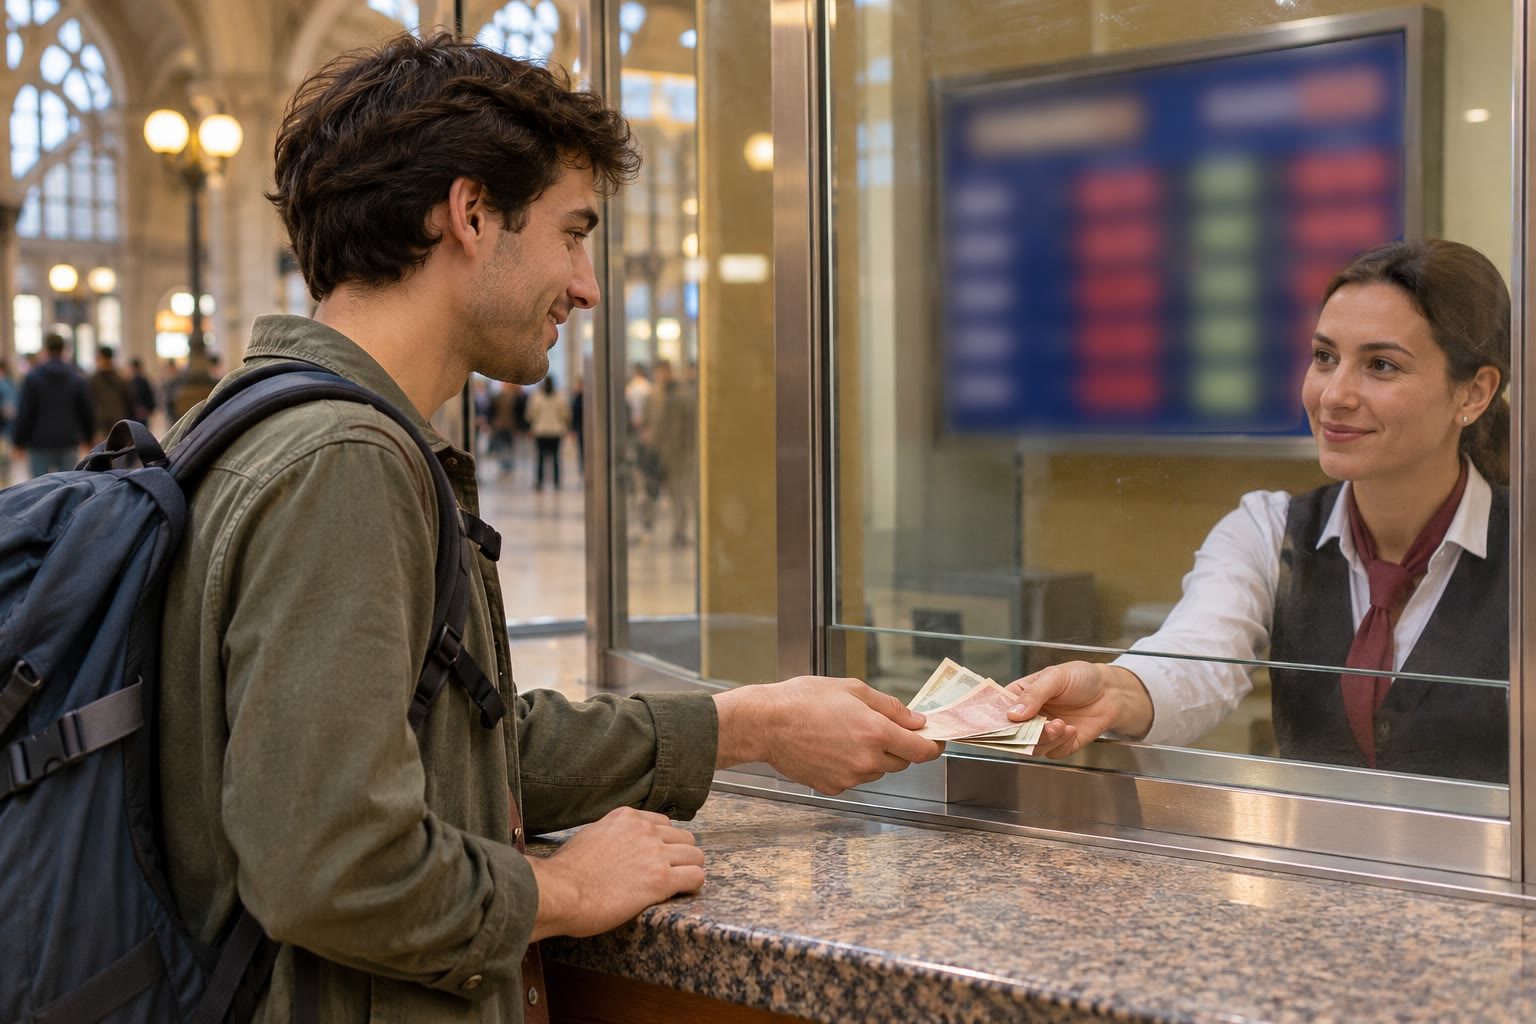
\includegraphics[width=0.48\linewidth]{images/book1/ai/g9-exchange-counter.jpg}

{\small A traveller changes \omterm{def:g7:money:money}{money} before a trip. The counter buys and sells currencies at a \omterm{def:g7:money:price}{price}.}
\end{omfigure}

\section{Converting amounts}

\begin{omfigure}
\begin{tikzpicture}[font=\small]
  \node[draw, rounded corners, minimum width=2.6cm, minimum height=1cm] (d) at (0,0) {dalens};
  \node[draw, rounded corners, minimum width=2.6cm, minimum height=1cm] (k) at (6,0) {kests};
  \draw[->, thick, omDef] (d.north east) to[bend left=20] node[above] {divide by $e$} (k.north west);
  \draw[->, thick, omThm] (k.south west) to[bend left=20] node[below] {multiply by $e$} (d.south east);
\end{tikzpicture}

{\small Converting between dalens and kests with $e = 1.242$ dalens per kest.}
\end{omfigure}

A meal that costs 20 kests in Kestria costs a Brenland traveller $20 \times 1.242 = 24.84$ dalens. With
100 dalens she gets $100 \div 1.242 = 80.52$ kests.

\section{When a currency rises or falls}

\begin{definition}[Appreciation]\label{def:g9:exchange-rates-and-purchasing-power:appreciation}
A \omterm{def:g9:exchange-rates-and-purchasing-power:currency}{currency} \emph{appreciates}\index{appreciation} when it buys more units of a foreign \omterm{def:g9:exchange-rates-and-purchasing-power:currency}{currency} than
before. For Brenland, the dalen appreciates when $e$ falls.
\end{definition}

\begin{definition}[Depreciation of a currency]\label{def:g9:exchange-rates-and-purchasing-power:depreciation}
A \omterm{def:g9:exchange-rates-and-purchasing-power:currency}{currency} \emph{depreciates}\index{depreciation (of a currency)} when it buys fewer units of a foreign
\omterm{def:g9:exchange-rates-and-purchasing-power:currency}{currency} than before. For Brenland, the dalen depreciates when $e$ rises.
\end{definition}

% figdata: brenland_rate (2024 1.207, 2025 1.242, +2.9 %)
In 2024 one kest cost 1.207 dalens; in 2025, 1.242. The kest became $2.9\,\%$ dearer: the dalen
depreciated. A Kestrian toy that costs 50 kests cost a Brenland shop $60.35$ dalens in 2024 and $62.10$
dalens in 2025, even though its \omterm{def:g7:money:price}{price} in kests did not change. In the other direction, a Brenland good of
100 dalens cost Kestrian buyers $82.85$ kests in 2024 and $80.52$ in 2025.

When a \omterm{def:g9:exchange-rates-and-purchasing-power:currency}{currency} \omterm{def:g9:exchange-rates-and-purchasing-power:depreciation}{depreciates}, the country's \omterm{def:g6:a-connected-world:import}{imports} become dearer at home and its \omterm{def:g6:a-connected-world:export}{exports} cheaper abroad:
it tends to buy fewer \omterm{def:g6:a-connected-world:import}{imports} and sell more \omterm{def:g6:a-connected-world:export}{exports}. When it \omterm{def:g9:exchange-rates-and-purchasing-power:appreciation}{appreciates}, the reverse.

\section{One basket, many prices}

\begin{definition}[Price level of a country]\label{def:g9:exchange-rates-and-purchasing-power:price-level}
The \emph{price level}\index{price level (of a country)} of a country, compared with another, is the cost
of a \omterm{def:g8:inflation-and-price-indices:basket}{basket} of goods and services in the first country, converted at the \omterm{def:g7:markets-and-prices:market}{market} \omterm{def:g9:exchange-rates-and-purchasing-power:exchange-rate}{exchange rate}, as a
percentage of the cost of the same \omterm{def:g8:inflation-and-price-indices:basket}{basket} in the second.
\end{definition}

\begin{model}{The law of one price}
\assumes A good can be shipped cheaply from one country to another, with no \omterm{def:g9:international-trade:tariff}{tariff} or other barrier.
\predicts Converted at the \omterm{def:g9:exchange-rates-and-purchasing-power:exchange-rate}{exchange rate}, the good costs about the same everywhere: if it were much
cheaper in one country, traders would buy it there and sell it in the other until the gap closed.
\tested For a \omterm{def:g8:inflation-and-price-indices:basket}{basket} of everything \omterm{def:g7:households:household}{households} buy, the prediction fails in a regular way: in 2024 the
\omterm{def:g9:exchange-rates-and-purchasing-power:price-level}{price level} of \omterm{def:g7:households:household}{household} consumption was below half of that of the United States in most countries with
less than 5,000 dollars per person (chart below).
\breaks Services that cannot be shipped (a haircut, a rent, a bus ride); \omterm{def:g9:international-trade:tariff}{tariffs} and transport costs; \omterm{def:g8:taxes-and-public-spending:tax}{taxes}
that differ from country to country.
\end{model}

% figdata: facts n_below_5000 31, pli_median_below_5000 35.4; n_above_50000 41, pli_median_above_50000 75.7
\begin{omchart}{Price level of household consumption (United States = 100) against GDP per person at
purchasing-power parity, 2024: one dot per country (171 countries).}{World \omterm{def:g8:banks-saving-interest:bank}{Bank}, World Development
Indicators (PA.NUS.PRVT.PLI and NY.GDP.PCAP.PP.CD)}
\begin{tikzpicture}
\begin{semilogxaxis}[omincomex, xmin=700, xmax=200000, ymin=0, ymax=180, width=0.85\linewidth,
  height=0.5\linewidth, xlabel={GDP per person at purchasing-power parity (dollars, times-ten scale)},
  ylabel={Price level (United States $=100$)}]
\addplot table[x=income, y=pli]
  {figdata/grade-9/05-exchange-rates-and-purchasing-power/out/price_level_income.csv};
\addplot[only marks, mark=*, mark size=1.8pt, omThm, nodes near coords, point meta=explicit symbolic,
  nodes near coords style={font=\scriptsize, text=black, anchor=south east}]
  table[x=income, y=pli, meta=label]
  {figdata/grade-9/05-exchange-rates-and-purchasing-power/out/price_level_named.csv};
\end{semilogxaxis}
\end{tikzpicture}
\end{omchart}

The dots rise from left to right. For the 31 countries with less than 5,000 dollars per person, the middle
\omterm{def:g9:exchange-rates-and-purchasing-power:price-level}{price level} is 35; for the 41 countries with more than 50,000, it is 76. Goods that are easily shipped,
such as phones, come closer to the law of one \omterm{def:g7:money:price}{price}. Services do not: a haircut in a poorer country is cut by a worker
who earns less, and it cannot be shipped to a richer country where haircuts are dear.

\section{Purchasing-power conversion}

\begin{definition}[Purchasing-power conversion]\label{def:g9:exchange-rates-and-purchasing-power:ppp}
A \emph{purchasing-power parity rate}\index{purchasing-power parity rate} (PPP rate) between two currencies
is the number of units of one \omterm{def:g9:exchange-rates-and-purchasing-power:currency}{currency} that buys the same \omterm{def:g8:inflation-and-price-indices:basket}{basket} of goods and services as one unit of the
other. Converting amounts with it is \emph{purchasing-power conversion}.
\end{definition}

If a \omterm{def:g8:inflation-and-price-indices:basket}{basket} costs 60 dalens in Brenland and 40 kests in Kestria, the PPP rate is $60 \div 40 = 1.5$ dalens
per kest. The \omterm{def:g7:markets-and-prices:market}{market} rate is 1.242: at the \omterm{def:g7:markets-and-prices:market}{market} rate, the \omterm{def:g8:inflation-and-price-indices:basket}{basket} bought in Kestria costs $40 \times
1.242 = 49.68$ dalens, less than in Brenland. Kestria's \omterm{def:g9:exchange-rates-and-purchasing-power:price-level}{price level}, compared with Brenland, is
$49.68 \div 60 = 82.8\,\%$.

\begin{measure}[Purchasing-power conversion]
% ledger: g9:icp-2021
The International Comparison Program, run by the World \omterm{def:g8:banks-saving-interest:bank}{Bank}, collects the \omterm{def:g7:money:price}{prices} of the same goods and
services in most countries of the world. Its latest round has 2021 as its reference year, and its results
were published in May 2024. From those \omterm{def:g7:money:price}{prices} it computes PPP rates and \omterm{def:g9:exchange-rates-and-purchasing-power:price-level}{price levels}; the values of other
years are estimated from them. \omterm{def:g8:gdp:gdp-per-person}{GDP per person} ``at purchasing-power parity'' is converted at these rates,
into dollars that buy in each country what a dollar buys in the United States.
\end{measure}

\begin{dated}{2026}
% ledger: g9:euro-members-2026
Several countries can share one \omterm{def:g9:exchange-rates-and-purchasing-power:currency}{currency}. In 2026 the euro is the \omterm{def:g9:exchange-rates-and-purchasing-power:currency}{currency} of 21 of the 27 member countries
of the European Union; the most recent to adopt it is Bulgaria, in 2026. Between those countries there is
no \omterm{def:g9:exchange-rates-and-purchasing-power:exchange-rate}{exchange rate} any more: a \omterm{def:g7:money:price}{price} in Lisbon and a \omterm{def:g7:money:price}{price} in Vienna can be compared directly.
\end{dated}

\section{Exercises}

\begin{exercise}[$\star$]\label{exo:g9:exchange-rates-and-purchasing-power:1}
In 2024 the United States' \omterm{def:g8:gdp:gdp-per-person}{GDP per person} was 86,170 dollars; India's was 2,592 dollars at \omterm{def:g7:markets-and-prices:market}{market} rates and
10,719 at purchasing-power parity. How many times larger was the United States' figure with each
conversion?
\end{exercise}

\begin{exercise}[$\star$]\label{exo:g9:exchange-rates-and-purchasing-power:2}
One kest costs $1.25$ dalens. How many kests does a traveller get for 500 dalens?
\end{exercise}

\begin{exercise}[$\star$]\label{exo:g9:exchange-rates-and-purchasing-power:3}
A Kestrian bicycle costs 80 kests. What does it cost in dalens when one kest costs $1.20$ dalens, and when
it costs $1.50$ dalens?
\end{exercise}

\begin{exercise}[$\star$]\label{exo:g9:exchange-rates-and-purchasing-power:4}
Read the \omterm{def:g9:exchange-rates-and-purchasing-power:price-level}{price levels} of Switzerland and India on the price-level chart. What does a \omterm{def:g8:inflation-and-price-indices:basket}{basket} that costs 100
dollars in the United States cost, converted into dollars, in each of them?
\end{exercise}

\begin{exercise}[$\star\star$]\label{exo:g9:exchange-rates-and-purchasing-power:5}
One kest cost $1.207$ dalens in 2024 and $1.242$ in 2025. By what percentage did the \omterm{def:g7:money:price}{price} of the kest
change? Did the dalen appreciate or depreciate?
\end{exercise}

\begin{exercise}[$\star\star$]\label{exo:g9:exchange-rates-and-purchasing-power:6}
A Brenland \omterm{def:g7:firms:firm}{firm} \omterm{def:g6:a-connected-world:import}{imports} a machine that costs 200 kests. One kest costs $1.20$ dalens. Then the dalen
\omterm{def:g9:exchange-rates-and-purchasing-power:depreciation}{depreciates} so that the kest costs $10\,\%$ more. Compute the machine's \omterm{def:g7:money:price}{price} in dalens before and after.
\end{exercise}

\begin{exercise}[$\star\star$]\label{exo:g9:exchange-rates-and-purchasing-power:7}
The dalen \omterm{def:g9:exchange-rates-and-purchasing-power:depreciation}{depreciates} against the kest. What happens to the \omterm{def:g7:money:price}{price} in kests of Brenland's \omterm{def:g6:a-connected-world:export}{exports}, and to the
\omterm{def:g7:money:price}{price} in dalens of its \omterm{def:g6:a-connected-world:import}{imports}? In which direction do \omterm{def:g6:a-connected-world:export}{exports} and \omterm{def:g6:a-connected-world:import}{imports} move?
\end{exercise}

\begin{exercise}[$\star\star$]\label{exo:g9:exchange-rates-and-purchasing-power:8}
A \omterm{def:g8:inflation-and-price-indices:basket}{basket} costs 300 dalens in Brenland and 250 kests in Kestria. Compute the PPP rate in dalens per kest.
\end{exercise}

\begin{exercise}[$\star\star$]\label{exo:g9:exchange-rates-and-purchasing-power:9}
One kest costs $1.25$ dalens. The same television costs 800 dalens in Brenland and 500 kests in Kestria.
Convert the Kestrian \omterm{def:g7:money:price}{price} into dalens. Does this observation contradict the law of one \omterm{def:g7:money:price}{price}? Give two
reasons why traders might not close the gap.
\end{exercise}

\begin{exercise}[$\star\star\star$]\label{exo:g9:exchange-rates-and-purchasing-power:10}
In an invented country, \omterm{def:g8:gdp:gdp-per-person}{GDP per person} is 2,000,000 zeds. The \omterm{def:g7:markets-and-prices:market}{market} rate is 100 zeds per dollar and the
PPP rate 40 zeds per dollar. Compute \omterm{def:g8:gdp:gdp-per-person}{GDP per person} in dollars with each rate. Which says more about what
people there can buy?
\end{exercise}

\begin{exercise}[$\star\star\star$]\label{exo:g9:exchange-rates-and-purchasing-power:11}
Explain why a haircut is usually cheaper, converted at the \omterm{def:g7:markets-and-prices:market}{market} rate, in a poorer country than in a
richer one, while a phone costs about the same.
\end{exercise}

\begin{exercise}[$\star\star\star$]\label{exo:g9:exchange-rates-and-purchasing-power:12}
Comparing \omterm{def:g8:gdp:gdp-per-person}{GDP per person} converted at \omterm{def:g7:markets-and-prices:market}{market} rates, does one overstate or understate how much poorer
the people of a poor country are than those of a rich one? Use the opening chart and the price-level
chart.
\end{exercise}

\section{Problem: A Summer in Kestria}

\begin{problem}[{Weekend problem --- converting a holiday budget, a moving exchange rate, and Brenland and
Kestria compared at market and at purchasing-power rates}]
\label{pb:g9:exchange-rates-and-purchasing-power:1}
Brenland and Kestria are invented. Mira, who lives in Brenland, spends her summer in Kestria. In 2025 one
kest costs $1.242$ dalens; in 2024 it cost $1.207$.

\medskip
\noindent\textbf{Part I --- The budget.}
\begin{enumerate}
  \item Mira has saved $2\,484$ dalens. How many kests does she get in 2025?
  \item A night in a youth hostel costs 30 kests. What is that in dalens?
  \item A meal costs 15 kests. What is that in dalens?
\end{enumerate}

\medskip
\noindent\textbf{Part II --- The rate moves.}
\begin{enumerate}[resume]
  \item Between 2024 and 2025, did the dalen appreciate or depreciate?
  \item By what percentage did the \omterm{def:g7:money:price}{price} of the kest change?
  \item What would $2\,000$ kests have cost Mira in 2024, and what do they cost in 2025?
\end{enumerate}

\medskip
\noindent\textbf{Part III --- Comparing the two countries.} A \omterm{def:g8:inflation-and-price-indices:basket}{basket} of bread, a bus ride, a haircut and a
cinema ticket costs 60 dalens in Brenland and 40 kests in Kestria.
\begin{enumerate}[resume]
  \item Compute the PPP rate in dalens per kest.
  \item Convert the Kestrian \omterm{def:g8:inflation-and-price-indices:basket}{basket} into dalens at the \omterm{def:g7:markets-and-prices:market}{market} rate. Where is the \omterm{def:g8:inflation-and-price-indices:basket}{basket} cheaper?
  \item Compute Kestria's \omterm{def:g9:exchange-rates-and-purchasing-power:price-level}{price level}, compared with Brenland, in percent.
  \item Kestria's \omterm{def:g8:gdp:gdp-per-person}{GDP per person} is $30\,000$ kests. Convert it into dalens at the \omterm{def:g7:markets-and-prices:market}{market} rate.
  \item Convert it into dalens at the PPP rate.
  \item Brenland's \omterm{def:g8:gdp:gdp-per-person}{GDP per person} in 2025 is $42\,327$ dalens. Compare it with your answers to questions 10
        and 11. Which country is richer per person, and which conversion should be used to compare what
        people can buy?
\end{enumerate}
\end{problem}
